\documentclass[11pt,a4paper]{article}
\usepackage[T1]{fontenc}
\usepackage[utf8]{inputenc}
\usepackage{lmodern}
\usepackage{helvet}
\renewcommand{\familydefault}{\sfdefault}
\usepackage[margin=2.15cm]{geometry}
\usepackage{xcolor}
\usepackage{hyperref}
\usepackage{booktabs}
\usepackage{enumitem}
\usepackage{fancyhdr}
\usepackage{titlesec}
\usepackage{caption}
\usepackage{graphicx}
\usepackage{float}
\usepackage{listings}
\usepackage{setspace}
\usepackage{microtype}
% Shared TikZ diagrams for LocalMesh Phase 1
\usepackage{tikz}
\usetikzlibrary{arrows.meta,calc,fit,positioning,shapes.geometric}

\definecolor{lmNavy}{HTML}{1B3A4B}
\definecolor{lmTeal}{HTML}{2A9D8F}
\definecolor{lmSand}{HTML}{E9C46A}
\definecolor{lmCoral}{HTML}{E76F51}
\definecolor{lmInk}{HTML}{264653}
\definecolor{lmMist}{HTML}{F4F1DE}
\definecolor{lmBlue}{HTML}{3D5A80}

\newcommand{\lmbox}[3]{%
  \node[draw=#1, fill=#1!12, line width=0.8pt, rounded corners=3pt,
        align=center, font=\scriptsize\sffamily, inner sep=5pt, #3] {#2};
}

\newcommand{\figcaptionstyle}{\captionsetup{font=small,labelfont={bf,sf},textfont=it}}

% ---------- Figure: LAN topology ----------
% Backends live INSIDE Your Mac (UTM). HTTPS is client -> Manohar first.
% The dashed arrow is DNS only (A-record), not the data path.
\newcommand{\drawTopology}{%
\begin{tikzpicture}[
  font=\sffamily\scriptsize,
  box/.style={draw=##1, fill=##1!10, line width=0.85pt, rounded corners=3pt,
              align=center, inner sep=5pt, minimum width=2.85cm, minimum height=1.25cm},
  lan/.style={draw=lmNavy, fill=lmNavy!6, rounded corners=6pt},
]
  \node[lan, minimum width=16.0cm, minimum height=7.35cm] (lan) at (0.15,0.05) {};
  \node[font=\sffamily\bfseries\small, text=lmNavy] at (0.15,3.25) {Private Wi-Fi / LAN  (two Macs + clients only)};

  \node[draw=lmNavy, fill=lmNavy!14, rounded corners=5pt, minimum width=7.5cm, minimum height=4.15cm] (host) at (-3.55,-0.45) {};
  \node[font=\sffamily\bfseries\scriptsize, text=lmNavy, anchor=north] at (-3.55,1.5) {Your Mac --- 10.7.12.104  (one Wi-Fi host)};

  \node[box=lmNavy] (dns) at (-3.55,0.55) {dnsmasq UDP/53\\answers \texttt{app.localmesh.test}};
  \node[box=lmBlue] (a) at (-5.15,-1.35) {\textbf{UTM guest A}\\not on Wi-Fi\\:3001 inside host};
  \node[box=lmCoral] (b) at (-1.95,-1.35) {\textbf{UTM guest B}\\not on Wi-Fi\\:3002 inside host};

  \node[box=lmTeal] (edge) at (4.55,1.05) {\textbf{Manohar's Mac}\\10.7.2.38\\nginx :8443};
  \node[box=lmSand, text=lmInk] (cli) at (4.55,-1.55) {\textbf{LAN client}\\browser / curl\\name, never backend IP};

  \draw[-{Latex}, lmNavy, densely dashed, thick] (dns.east) -- node[above, font=\tiny, align=center] {DNS A-record only\\not HTTPS} (edge.west);
  \draw[-{Latex}, lmTeal, very thick] (cli) -- node[right, font=\tiny] {1. HTTPS :8443} (edge);
  \draw[-{Latex}, lmBlue, thick] (edge.south west) -- node[below, font=\tiny, sloped, pos=0.45] {2. proxy 10.7.12.104:3001/3002} (host.east);
\end{tikzpicture}%
}

% ---------- Figure: request path ----------
\newcommand{\drawRequestPath}{%
\begin{tikzpicture}[font=\sffamily\tiny, node distance=0.35cm and 0.28cm]
  \tikzset{s/.style={draw=##1, fill=##1!14, rounded corners=2pt, align=center,
           inner sep=4pt, minimum height=1.05cm, minimum width=2.15cm, line width=0.7pt}}
  \node[s=lmNavy] (1) {1. DNS query\\UDP/53\\10.7.12.104};
  \node[s=lmTeal, right=of 1] (2) {2. A record\\app.localmesh.test\\$\to$ 10.7.2.38};
  \node[s=lmBlue, right=of 2] (3) {3. TCP\\SYN / SYN-ACK / ACK\\:8443};
  \node[s=lmSand, right=of 3] (4) {4. TLS 1.3\\team CA\\app cert};
  \node[s=lmCoral, right=of 4] (5) {5. HTTP/2\\nginx $\to$\\10.7.12.104:3001/2};
  \foreach \a/\b in {1/2,2/3,3/4,4/5}
    \draw[-{Latex}, thick, lmInk] (\a) -- (\b);
\end{tikzpicture}%
}

% ---------- Figure: UTM forwards ----------
\newcommand{\drawUtm}{%
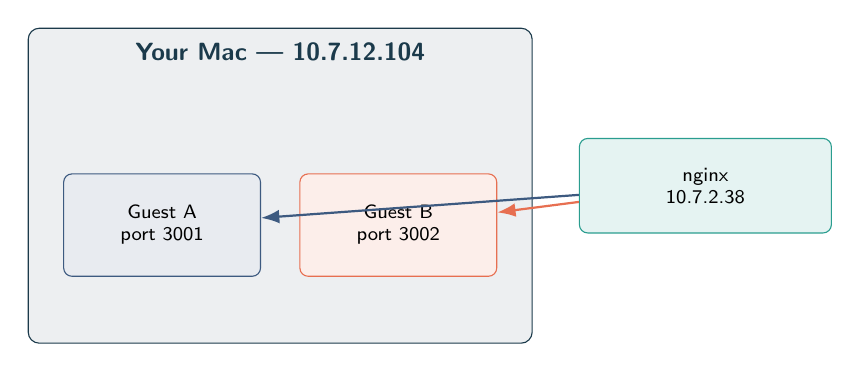
\begin{tikzpicture}[font=\sffamily\scriptsize]
  \node[draw=lmNavy, fill=lmNavy!8, rounded corners=4pt, minimum width=6.4cm, minimum height=4.0cm] (host) at (0,0) {};
  \node[font=\bfseries\small, text=lmNavy] at (0,1.7) {Your Mac --- 10.7.12.104};
  \node[draw=lmBlue, fill=lmBlue!12, rounded corners=3pt, align=center, minimum width=2.5cm, minimum height=1.3cm] (va) at (-1.5,-0.5) {Guest A\\port 3001};
  \node[draw=lmCoral, fill=lmCoral!12, rounded corners=3pt, align=center, minimum width=2.5cm, minimum height=1.3cm] (vb) at (1.5,-0.5) {Guest B\\port 3002};
  \node[draw=lmTeal, fill=lmTeal!12, rounded corners=3pt, align=center, minimum width=3.2cm, minimum height=1.2cm] (ng) at (5.4,0) {nginx\\10.7.2.38};
  \draw[-Latex, thick, lmBlue] (ng) -- (va);
  \draw[-Latex, thick, lmCoral] (ng) -- (vb);
\end{tikzpicture}%
}

% ---------- Figure: TLS chain ----------
\newcommand{\drawTls}{%
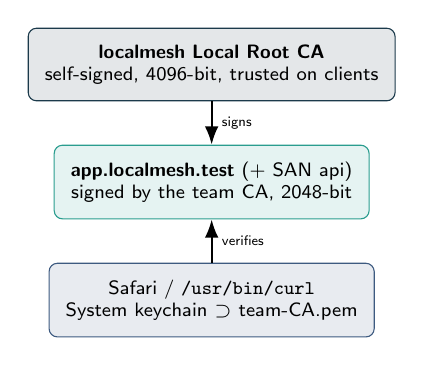
\begin{tikzpicture}[font=\sffamily\scriptsize, node distance=0.55cm]
  \node[draw=lmNavy, fill=lmNavy!12, rounded corners=3pt, align=center, inner sep=6pt] (ca)
    {\textbf{localmesh Local Root CA}\\self-signed, 4096-bit, trusted on clients};
  \node[draw=lmTeal, fill=lmTeal!12, rounded corners=3pt, align=center, inner sep=6pt, below=of ca] (srv)
    {\textbf{app.localmesh.test} (+ SAN api)\\signed by the team CA, 2048-bit};
  \node[draw=lmBlue, fill=lmBlue!12, rounded corners=3pt, align=center, inner sep=6pt, below=of srv] (cli)
    {Safari / \texttt{/usr/bin/curl}\\System keychain $\supset$ team-CA.pem};
  \draw[-{Latex}, thick] (ca) -- node[right, font=\tiny] {signs} (srv);
  \draw[-{Latex}, thick] (cli) -- node[right, font=\tiny] {verifies} (srv);
\end{tikzpicture}%
}

% ---------- Figure: OSI mapping ----------
\newcommand{\drawOsi}{%
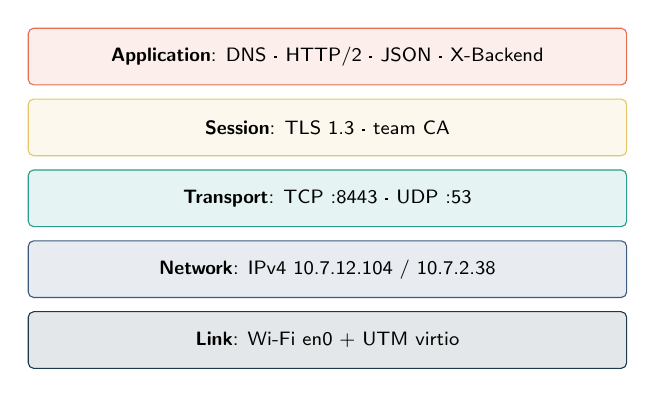
\begin{tikzpicture}[font=\sffamily\scriptsize]
  \foreach \y/\c/\t/\n in {
    4.2/lmCoral/Application/{DNS · HTTP/2 · JSON · X-Backend},
    3.3/lmSand/Session/{TLS 1.3 · team CA},
    2.4/lmTeal/Transport/{TCP :8443 · UDP :53},
    1.5/lmBlue/Network/{IPv4 10.7.12.104 / 10.7.2.38},
    0.6/lmNavy/Link/{Wi-Fi en0 + UTM virtio}
  } {
    \node[draw=\c, fill=\c!12, rounded corners=2pt, minimum width=7.6cm,
          minimum height=0.72cm, anchor=west] at (0,\y) {\textbf{\t}: \n};
  }
\end{tikzpicture}%
}


\hypersetup{
  colorlinks=true,
  linkcolor=lmNavy,
  urlcolor=lmTeal,
  pdftitle={LocalMesh Phase 1 Report},
  pdfauthor={Harsith, Manohar}
}

\titleformat{\section}{\Large\bfseries\color{lmNavy}}{\thesection}{0.6em}{}
\titleformat{\subsection}{\large\bfseries\color{lmTeal}}{\thesubsection}{0.5em}{}
\titleformat{\subsubsection}{\normalsize\bfseries\color{lmInk}}{\thesubsubsection}{0.4em}{}

\pagestyle{fancy}
\fancyhf{}
\fancyhead[L]{\small LocalMesh --- Phase 1 report}
\fancyhead[R]{\small Computer Networks}
\fancyfoot[C]{\thepage}
\renewcommand{\headrulewidth}{0.4pt}

\lstset{
  basicstyle=\ttfamily\footnotesize,
  frame=single,
  rulecolor=\color{lmNavy!30},
  backgroundcolor=\color{lmNavy!4},
  breaklines=true,
  columns=fullflexible,
  keepspaces=true
}

\setlist{itemsep=3pt, topsep=4pt}
\setstretch{1.12}

\begin{document}

\begin{titlepage}
\pagecolor{lmNavy}
\color{white}
\vspace*{1.6cm}
{\Huge\bfseries LocalMesh}\\[8pt]
{\LARGE Private Network Service Platform}\\[18pt]
{\color{lmTeal}\rule{4.2cm}{2.4pt}}\\[16pt]
{\Large Phase 1 report}\\[6pt]
{\large Build and observe the network}\\[2.4cm]
\begin{tabular}{@{}ll}
  \color{lmTeal} Course & \color{white} Computer Networks \\[4pt]
  \color{lmTeal} Review & \color{white} Phase 1 / Review 1 \\[4pt]
  \color{lmTeal} Zone & \color{white} \texttt{localmesh.test} \\[4pt]
  \color{lmTeal} Authors & \color{white} Harsith (DNS, UTM host) \\
                         & \color{white} Manohar (nginx, TLS, edge) \\[4pt]
  \color{lmTeal} IPs & \color{white} 10.7.12.104 \quad 10.7.2.38 \\
\end{tabular}
\vfill
{\small The application stays simple --- the network is the project.}
\end{titlepage}
\nopagecolor
\color{black}

\tableofcontents
\newpage

\section{Abstract}
LocalMesh is a fully local private service: a client types \texttt{https://app.localmesh.test:8443},
resolves the name through the team's own DNS, completes TLS at a reverse proxy, and receives JSON
from one of two backend processes. Phase~1 implements four network roles on two physical Macs.
Your Mac (\texttt{10.7.12.104}) runs dnsmasq and hosts two Ubuntu guests in UTM Emulated VLAN.
Manohar's Mac (\texttt{10.7.2.38}) terminates TLS and load-balances to
\texttt{10.7.12.104:3001} and \texttt{:3002}. This report records the architecture, protocol
mapping, configuration, observations, and failure analysis required for Review~1.
It is the commitable Phase~1 document. Machine-by-machine setup runbooks stay out of git.

\section{Purpose and constraints}
The brief asks for a private environment with no cloud. A client must (i)~use a \texttt{.test}
name, (ii)~hit the team DNS, (iii)~open HTTPS on the team edge, (iv)~see both backends through
the load balancer, and (v)~show the path in packet captures. Ports 8080/8443 may replace 80/443.
Teams of two or three may combine hardware as long as the four \emph{roles} exist.

We chose Option~A: both backends on Your Mac. That is allowed. Emulated VLAN plus port
forwarding is a hypervisor feature; it is not ``implementing NAT'' as a course topic.
Phase~1 explicitly does not require student-built NAT, VLANs, or routing protocols.

\section{Architecture}

\subsection{Roles versus hardware}
\begin{table}[h]
\centering
\caption{Mapping from the brief to this team.}
{\small
\begin{tabular}{@{}llll@{}}
\toprule
\textbf{Brief} & \textbf{This team} & \textbf{LAN identity} & \textbf{Software} \\
\midrule
Mac 1 DNS + client & Your Mac & 10.7.12.104 & dnsmasq :53 \\
Mac 2 edge + TLS + LB & Manohar's Mac & 10.7.2.38 & nginx :8080/:8443 \\
Mac 3 Backend A & UTM VM, forward 3001 & 10.7.12.104:3001 & Python A \\
Mac 4 Backend B + client & UTM LocalMesh-1, forward 3002 & 10.7.12.104:3002 & Python B \\
\bottomrule
\end{tabular}}
\end{table}

Shared settings live only on each machine in \texttt{\textasciitilde/cn-team.env}
(\texttt{TEAM=localmesh}). They are not committed.

\subsection{LAN topology}
\begin{figure}[H]
\centering
\resizebox{\textwidth}{!}{\drawTopology}
\caption{Wi-Fi has two Macs. Backends are UTM guests inside Your Mac, not LAN hosts. Dashed arrow = DNS A-record only. HTTPS is always client $\to$ Manohar :8443, then proxy to 10.7.12.104:3001 or :3002.}
\end{figure}

Clients always use the name. nginx is the only process they should treat as ``the service''.
The dashed Your-Mac--to--Manohar arrow is \textbf{not} the HTTPS path; it is the DNS answer
\texttt{app.localmesh.test $\mapsto$ 10.7.2.38}. Browsers then open TCP to Manohar :8443.
Guests sit on UTM's user-mode VLAN (classically \texttt{10.0.2.0/24}). They are not extra
Wi-Fi IPs. Manohar cannot ping those addresses. He reaches backends only as
\texttt{10.7.12.104:3001} and \texttt{:3002}.

\subsection{Request path}
\begin{figure}[H]
\centering
\resizebox{\textwidth}{!}{\drawRequestPath}
\caption{One successful client request, left to right.}
\end{figure}

\subsection{UTM publication}
UTM Shared Network never shows a Port Forward table. Emulated VLAN does.
Host Address must be the Wi-Fi IPv4, not blank (blank binds loopback only).

\begin{figure}[H]
\centering
\resizebox{0.92\textwidth}{!}{\drawUtm}
\caption{nginx talks only to Your Mac's published ports.}
\end{figure}

\section{Protocol layers}

\begin{figure}[H]
\centering
\drawOsi
\caption{Classroom stack mapped onto LocalMesh.}
\end{figure}

\paragraph{DNS.}
dnsmasq listens on \texttt{127.0.0.1} and \texttt{10.7.12.104}.
\texttt{local=/localmesh.test/} means that zone is never forwarded.
\texttt{host-record} creates A and PTR for \texttt{app} and \texttt{api} to \texttt{10.7.2.38}.
Other names go to \texttt{8.8.8.8} and \texttt{1.1.1.1}. Evidence: \texttt{dig} SERVER
\texttt{10.7.12.104\#53}, answer \texttt{10.7.2.38}.

\paragraph{TCP.}
After resolution the client opens \texttt{10.7.2.38:8443}. Capture the SYN, SYN-ACK, ACK
before any application data. Source port is ephemeral; destination is 8443 (or 53 for DNS).

\paragraph{TLS.}
\begin{figure}[H]
\centering
\drawTls
\caption{Private CA. Clients must trust \texttt{team-CA.pem}. Use \texttt{/usr/bin/curl}, never \texttt{-k}.}
\end{figure}

Observed: TLSv1.3, issuer \texttt{CN=localmesh Local Root CA}.

\paragraph{HTTP and caching.}
Backends return JSON and \texttt{X-Backend}. \texttt{Cache-Control: max-age=60}.
ETags differ (\texttt{backend-a-v1} vs \texttt{backend-b-v1}), so a 304 through the
load balancer is not reliable. Review~1 can still show the headers. \texttt{curl -I}
sends HEAD; these apps implement GET only, so HEAD on \texttt{/} is HTTP/1.0 501.
Use GET (or \texttt{curl -D - -o /dev/null}) for status evidence.

\paragraph{Load balancing.}
nginx \texttt{upstream} lists both host ports, default round-robin, \texttt{max\_fails=1}.
Repeated \texttt{/api/status} must show both A and B while both processes run.

\section{Implementation (what we built, not a runbook)}

\subsection{Private DNS}
Homebrew dnsmasq on Your Mac. Wi-Fi clients set their resolver to \texttt{10.7.12.104}.
\texttt{.test} avoids Bonjour \texttt{.local}. Upstream servers keep the ordinary internet working
while the private zone stays local.

\subsection{Backends}
Two Python 3 \texttt{http.server} apps bind \texttt{0.0.0.0} (required so the hypervisor can
forward). Endpoints: \texttt{GET /} and \texttt{GET /api/status}. Code is in
\texttt{backend-a/app.py} and \texttt{backend-b/app.py}.

\subsection{Edge}
nginx on Manohar's Mac. HTTP 8080 redirects to HTTPS 8443. \texttt{proxy\_pass} to
\texttt{http://backends}. \texttt{proxy\_next\_upstream} covers a dead member.

\subsection{TLS}
A 4096-bit team CA signs the server certificate. SAN lists both names. Every client
installs the CA as a trust anchor. That is how a padlock appears without a public CA.

\section{Observations and evidence}
Filed under \texttt{evidence/phase1/} (see \texttt{INDEX.md}):

\begin{itemize}
  \item DNS config and \texttt{dig} (zone, A records, SERVER line).
  \item Ping of both Macs; direct HTTP to :3001 and :3002 with A/B headers.
  \item HTTPS verbose: TLS 1.3, team CA issuer, mixed \texttt{x-backend}.
  \item Browser on \texttt{app.localmesh.test:8443} returning JSON.
  \item Guests listening on \texttt{0.0.0.0:3001} and \texttt{:3002}.
  \item \texttt{flow.pcap} (UDP/53 and TCP/8443).
  \item F1: client resolver set to 8.8.8.8 $\Rightarrow$ NXDOMAIN for \texttt{app.localmesh.test}.
\end{itemize}

Still to add before the slot if missing: Wireshark stills from the pcap (DNS, handshake, ClientHello);
F2 wrong A record; F3 one backend stopped; F4 both stopped (502); F5 wrong port;
\texttt{openssl verify}.

\section{Failure analysis}
These are required Phase~1 demonstrations. They isolate layers.

\begin{table}[h]
\centering
\caption{Deliberate faults and the layer they expose.}
{\small
\begin{tabular}{@{}p{3.4cm}p{5.4cm}p{5.4cm}@{}}
\toprule
\textbf{Fault} & \textbf{Observation} & \textbf{Lesson} \\
\midrule
Wrong client DNS (8.8.8.8) & NXDOMAIN; IP ping still works & Name and reachability are independent \\
Wrong A record & \texttt{dig} succeeds, TCP/TLS to the wrong host fails & DNS is a directory \\
One backend stopped & Remaining \texttt{X-Backend} only & Edge continues; HA is incomplete without health checks in the demo path \\
Both backends stopped & 502 from nginx & Edge is up; origin is not \\
Wrong destination port & Connection refused / timeout on :9999 & IP $\neq$ service \\
\bottomrule
\end{tabular}}
\end{table}

Diagnosis order if faculty inject a fault: (1)~name, (2)~TCP to :8443,
(3)~TLS/issuer, (4)~JSON/\texttt{X-Backend}.

\section{Learning notes (viva)}
\begin{itemize}
  \item DNS finds an IP. TCP then builds a connection. TLS then authenticates the name.
  \item Clients must not skip the edge. Direct :3001/:3002 is only for proving the LAN.
  \item Two backends share one host IP because UTM publishes them as ports, not as extra LAN NICs.
  \item Trusting \texttt{app.crt} is wrong; trusting the CA is right.
  \item \texttt{.local} would never reach dnsmasq.
\end{itemize}

\section{What is not in this repository}
Detailed paste-this-next setup guides stay in the private \texttt{docs/} folder (gitignored).
They are operational notes, not the academic deliverable. This report, \texttt{config/},
backend source, and \texttt{evidence/} are what Review~1 should see.

\section{Conclusion}
Phase~1 is a working private name, a trusted HTTPS edge, two identifiable backends, and
packet-level proof of DNS, TCP, and TLS. The topology uses two Macs honestly and still
presents four roles. Phase~2 (backup DNS, isolation, TTL, cutover) extends this system;
it is not part of this report.

\appendix
\section{Reference configuration}
Values match a live \texttt{\textasciitilde/cn-team.env}. Private keys are not included.

\subsection{dnsmasq (excerpt)}
\begin{lstlisting}
listen-address=127.0.0.1,10.7.12.104
no-resolv
server=8.8.8.8
local=/localmesh.test/
host-record=app.localmesh.test,10.7.2.38
host-record=api.localmesh.test,10.7.2.38
\end{lstlisting}

\subsection{nginx upstream (excerpt)}
\begin{lstlisting}
upstream backends {
    server 10.7.12.104:3001 max_fails=1 fail_timeout=10s;
    server 10.7.12.104:3002 max_fails=1 fail_timeout=10s;
}
\end{lstlisting}

\subsection{Backend contract}
\texttt{GET /api/status} $\rightarrow$ \texttt{\{"backend": "A"|"B", "status": "ok"\}}
and header \texttt{X-Backend}.

\end{document}
